
\section{Circuits}
Turing machines are rather idealized models of computing devices. Real computers are finite in size, whereas for Turing machines we assumed a computer of unbounded size. The Circuits model provides a more realistic way of making a real computer.\\
A circuit is made up of wires and gates, which carry information around, and perform simple computational tasks, respectively. A circuit may involve multiple input and output bits, many wires, and many logical gates. A logic gate is a function f : {$\{0, 1\}^k \longmapsto \{0, 1\}^l$} from some fixed number k of input bits to some fixed number l of output bits.\\
The following image shows the standard symbols for each of the elementary gates along with there truth tables.\\
\begin{figure}[h!]	
	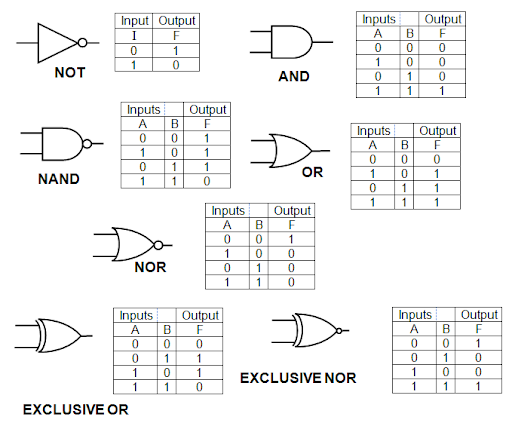
\includegraphics[width=1\textwidth]{images/gate.png}\par
	\caption{Elementary gates}
	\label{fig:gate}
\end{figure}
\\Along with these gates there are two more gates, {\scshape Fanout} and {\scshape Crossover}. {\scshape Fanout} is gate used to duplicate a bit or rather 'divide' a bit into two with same value. {\scshape Crossover} is used to interchange the values of two bits.\\
These basic gates can be combined to do a large number of operations. Actually, these gates can be used to compute any function f:{$\{0, 1\}^n \longmapsto \{0, 1\}^n$}. Moreover, among these elementary gates, {\scshape NAND} and {\scshape NOR} are called {\bf Universal Gates} as they can be used to simulate other elementary gates (given wires, ancilla and {\scshape Fanout} is available.) As an example the image below shows the circuit used to add two binary numbers:\\
\begin{figure}[h]	
	\begin{subfigure}[b]{0.5\linewidth}
	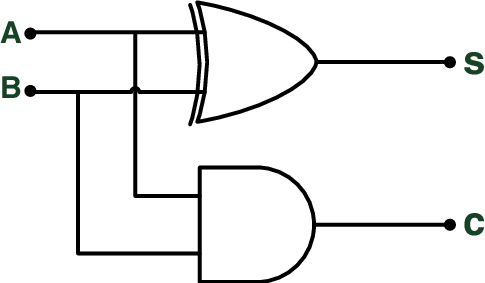
\includegraphics[width=1\textwidth]{images/halfadder.png}\par
	\caption{the circuit for a half adder}
 	\end{subfigure}
	\begin{subfigure}[b]{0.5\linewidth}
	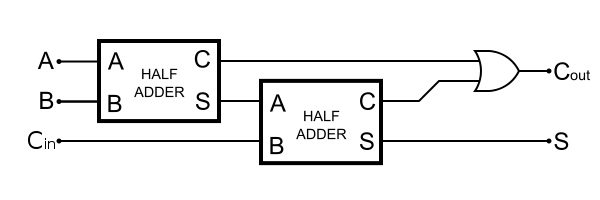
\includegraphics[width=1\textwidth]{images/fulladder.png}\par
	\caption{full adder from two half adder circuits}
 	\end{subfigure}
\label{fig:gate}
\caption{Circuit to add two binary numbers}
\end{figure}
\subsection{Circuit Families}
A {\bf Circuit Family} consists of a collection of circuits, {$ \{C_n \} $}, indexed by a positive integer n. The circuit {$C_n$} has n input bits, and may have any finite number of extra work bits, and output bits. The output of the circuit {$C_n$} , upon input of a number x of at most n bits in length, is denoted by {$C_n$}(x). We require that the circuits be consistent, that is, if {$m < n$} and x is at most m bits in length, then {$C_m$}(x) = {$C_n$}(x). The function computed by the circuit family {$ \{C_n\}$} is the function C({$\cdotp$}) such that if x is n bits in length then C(x) = {$C_n$}(x).
\\A family of circuits {$ \{C_n \} $} is said to be a {\bf uniform circuit family} if there is some algorithm running on a Turing machine which, upon input of n, generates a description of {$ C_n $}. That is, the algorithm outputs a description of what gates are in the circuit {$ C_n $} , how those gates are connected together to form a circuit, any ancilla bits needed by the circuit, {\scshape Fanout} and {\scshape Crossover} operations, and where the output from the circuit should be read out. In simple terms, there must exist a definite algorithmic way in which an engineer can construct a circuit for {$ \{C_n \} $} for any n.\\
With this uniformity restriction, results in the Turing machine model of computation can usually be given a straightforward translation into the circuit model of computation, and vice versa.
\newpage
